\section{从相关到独立}
\label{sec:dep-correlation-to-independence}

协方差为零时，两个变量还可能有多强的联系？先把开头的抛物线算清楚。

\paragraph{零协方差的抛物线}
设$X\sim\operatorname{Unif}(-1,1)$，$Y=X^{2}$。$X$的密度在$[-1,1]$上为$1/2$，奇数次矩为零，于是
\[
  \mathbb{E}[X]=0,\qquad \mathbb{E}[X^{3}]=\frac12\int_{-1}^{1}x^{3}\,\mathrm{d}x=0 .
\]
代入协方差的定义，得到
\[
  \operatorname{Cov}(X,Y)=\mathbb{E}[XY]-\mathbb{E}[X]\,\mathbb{E}[Y]=\mathbb{E}[X^{3}]-0=0 .
\]
$X$与$Y$不相关。但它们并不独立：事件$A=\{\lvert X\rvert\leq1/2\}$发生时一定有$Y\leq1/4$，所以
\[
  \mathbb{P}\bigl(\lvert X\rvert\leq\tfrac12,\ Y>\tfrac14\bigr)=0 .
\]
若两者独立，这个概率应当等于两个边缘概率的乘积，
\[
  \mathbb{P}\bigl(\lvert X\rvert\leq\tfrac12\bigr)\,\mathbb{P}\bigl(Y>\tfrac14\bigr)=\frac12\cdot\frac12=\frac14 .
\]

图~\ref{fig:dep-parabola-joint-product}把这两个数画了出来。左图是$(X,Y)$的样本，全部落在抛物线上；右图是“假装独立”的样本：$X$与$Y$各按自己的边缘分布抽取，但彼此独立。两幅图的横坐标分布相同，纵坐标分布也相同，差别只在点怎样配对。红框里的事件在左图中没有点，在右图中约占四分之一。

\begin{BookInlineFigure}
  \centering
  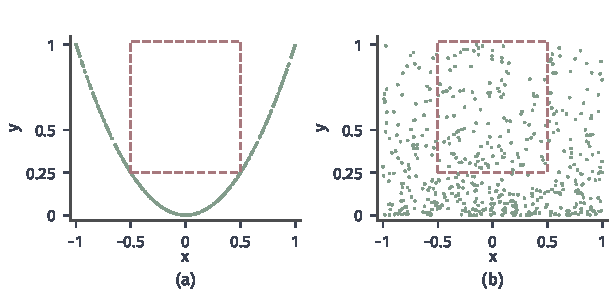
\includegraphics[width=104mm]{figures/07-probability/04-distribution-analysis/matplotlib/dep-parabola-joint-product/figure.pdf}
  \caption{同样的边缘，不同的配对。(a)$X\sim\operatorname{Unif}(-1,1)$，$Y=X^{2}$的$500$个样本（绿）；(b)边缘乘积$P_X\otimes P_Y$的$500$个样本，即把$X$与一个独立复制$X'$的平方配对。红色虚线框是事件$\{\lvert x\rvert\leq1/2,\ y>1/4\}$，其概率在(a)中为$0$，在(b)中为$1/4$（样本中占$0.248$）。种子$719$。}
  \label{fig:dep-parabola-joint-product}
\end{BookInlineFigure}

\paragraph{协方差只是一个测试}
协方差为零说的是$\mathbb{E}[(X-\mathbb{E}X)(Y-\mathbb{E}Y)]=0$，即一对特定函数$x\mapsto x$、$y\mapsto y$的乘积在联合分布下的期望，与在边缘乘积下的期望相同。独立要求的多得多：对一切有界可测函数$f,g$，
\begin{equation}
  \mathbb{E}\bigl[f(X)\,g(Y)\bigr]=\mathbb{E}\bigl[f(X)\bigr]\,\mathbb{E}\bigl[g(Y)\bigr],
  \label{eq:dep-independence-test-functions}
\end{equation}
这等价于联合分布等于边缘乘积，
\begin{equation}
  P_{(X,Y)}=P_X\otimes P_Y .
  \label{eq:dep-independence}
\end{equation}
取$f,g$为示性函数，式~\eqref{eq:dep-independence-test-functions}就是矩形事件上的乘积公式，它确定两个分布相等；反过来，由矩形事件的乘积公式经简单函数逼近得到一般有界$f,g$的情形，这正是第~\ref{chap:probability-spaces}章建立独立性时走过的路。

协方差是式~\eqref{eq:dep-independence-test-functions}中只取一对线性函数的结果，换一对函数就能看出抛物线的依赖。取$f(x)=x^{2}$，$g(y)=y$，由$\mathbb{E}[X^{2}]=1/3$与$\mathbb{E}[X^{4}]=1/5$，
\[
  \operatorname{Cov}\bigl(X^{2},Y\bigr)=\operatorname{Var}\bigl(X^{2}\bigr)=\frac15-\frac19=\frac{4}{45}>0 .
\]
所以“协方差为零”只排除了一种线性的联系。这一点在第~\ref{chap:random-vectors}章已经见过：不相关不等于独立。

\paragraph{零相关的几种形状}
图~\ref{fig:dep-zero-correlation-shapes}收集了几种协方差为零的联合分布。(b)中$Y=SX$，$S$是与$X$独立、等可能取$\pm1$的随机符号，协方差是$\mathbb{E}[S]\,\mathbb{E}[X^{2}]=0$，可是$\lvert Y\rvert=\lvert X\rvert$。(c)是单位圆周上的均匀分布，两个坐标满足$X^{2}+Y^{2}=1$。只有(d)两个坐标独立。四幅图的相关系数都是零，相关系数无法把(d)与前三幅区分开。

\begin{BookInlineFigure}
  \centering
  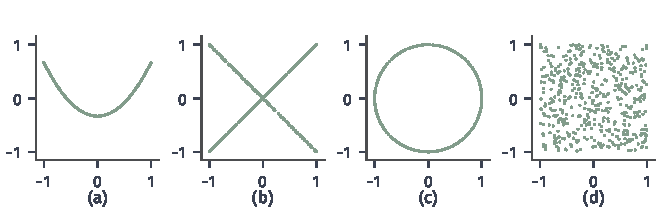
\includegraphics[width=112mm]{figures/07-probability/04-distribution-analysis/matplotlib/dep-zero-correlation-shapes/figure.pdf}
  \caption{协方差都为零的四个联合分布，各$500$个样本（种子$719$）。(a)$X\sim\operatorname{Unif}(-1,1)$与$X^{2}-1/3$；(b)$X$与$SX$，$S$为独立随机符号；(c)单位圆周上的均匀分布；(d)两个独立的$\operatorname{Unif}(-1,1)$。前三个都不独立。}
  \label{fig:dep-zero-correlation-shapes}
\end{BookInlineFigure}

\paragraph{相关足够的两种情形}
有两类联合分布，零相关确实等价于独立。一类是联合高斯向量，第~\ref{chap:multivariate-distributions}章已经证明。另一类是两个二值变量。设$X,Y$都取值于$\{0,1\}$，记$p=\mathbb{P}(X=1)$，$q=\mathbb{P}(Y=1)$。由$XY=\mathbf{1}_{\{X=1,Y=1\}}$，
\[
  \mathbb{P}(X=1,\,Y=1)-pq=\mathbb{E}[XY]-\mathbb{E}[X]\,\mathbb{E}[Y]=\operatorname{Cov}(X,Y).
\]
其余三个格子由边缘减出来。例如$\mathbb{P}(X=1,Y=0)=p-\mathbb{P}(X=1,Y=1)$，它与$p(1-q)$之差是$-\operatorname{Cov}(X,Y)$。所以$2\times2$概率表的四个格子与独立时的乘积只差$\pm\operatorname{Cov}(X,Y)$，协方差为零时四个格子都分解成乘积。二值变量只有一个“自由度”可以偏离独立，协方差恰好量的就是它。取值多于两个时，偏离独立的方向不止一个，单个协方差看不全。

\paragraph{三点抛物线}
最小的反例只需要三个点。设$X$在$\{-1,0,1\}$上等可能，$Y=X^{2}$。$(X,Y)$等可能取$(-1,1)$、$(0,0)$、$(1,1)$三个值，边缘为
\[
  \mathbb{P}(X=x)=\tfrac13\ (x=-1,0,1),\qquad \mathbb{P}(Y=1)=\tfrac23,\qquad \mathbb{P}(Y=0)=\tfrac13 .
\]
协方差仍是$\mathbb{E}[X^{3}]=\frac13(-1+0+1)=0$。图~\ref{fig:dep-three-point-tables}把联合概率表与边缘乘积表并排放在一起：联合表有三个格子为零，乘积表六个格子都是正数。这个例子取值有限，所有度量都能手算，后面每一节都会回到它。

\begin{BookInlineFigure}
  \centering
  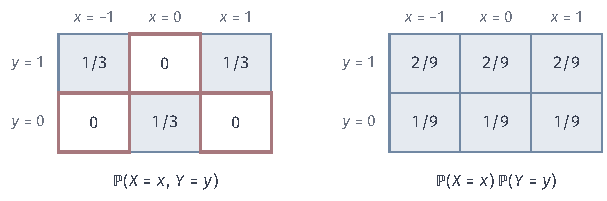
\includegraphics[width=102.8mm]{figures/07-probability/04-distribution-analysis/tikz/dep-three-point-tables/figure.pdf}
  \caption{三点抛物线。左：联合概率表$\mathbb{P}(X=x,Y=y)$，浅蓝格子有正质量，红框标出联合表为零而乘积表为正的三个格子。右：边缘乘积$\mathbb{P}(X=x)\,\mathbb{P}(Y=y)$，其中$\mathbb{P}(Y=1)=2/3$，$\mathbb{P}(Y=0)=1/3$。}
  \label{fig:dep-three-point-tables}
\end{BookInlineFigure}

\paragraph{依赖度量要回答的三件事}
于是共同的问题是：$P_{(X,Y)}$离$P_X\otimes P_Y$有多远。把联合分布映成一个非负数的泛函，称为\term{依赖度量}（dependence measure）。评价一个依赖度量，要把三件不同的事分开。

第一件是零值判据：度量为零是否当且仅当独立。协方差在一般分布上做不到，在联合高斯和二值变量上做得到；本章的互信息、距离协方差、高斯核HSIC在各自的条件下都做得到。第二件是非零数值的含义：依赖变强时数值是否增大，有没有上界，对重新标记、平移、缩放、单调变换是否敏感，需要预先选哪些参数。这一件没有统一答案，不同度量给同一对分布排出的强弱次序可以相反。第三件是有限样本：只观测到$n$对数据时，能否可靠地判断度量是否为零，误差有多大。

本章的定义都是总体量，只回答前两件事。第三件要另外分析估计量的偏差、方差和分布，即使度量的零值完全刻画独立，样本上算出的一个正数也不等于证明了依赖，这部分由统计推断承担，可参考\BookChapterRef{chap:nonparametric-inference}{卷八第2章“非参数分布与函数推断”}。
